\documentclass[a4paper]{article}
\usepackage[spanish]{babel}
\usepackage{graphicx}
\pagestyle{headings}
\titlepage
\usepackage[utf8]{inputenc} 		% para codificacion unicode (utf8)
\usepackage{enumerate}
\usepackage{hyperref}			% para links a paginas web
\usepackage{subfig}
\usepackage{graphics}
\usepackage{amsmath}
\usepackage{amssymb}
\usepackage{amsthm}
\usepackage{placeins}
%\usepackage{tabularx}
\usepackage{booktabs,siunitx}
%\usepackage{fullpage}

\decimalpoint

% That follow if for listings configuration
\usepackage{listings}
\usepackage{color}
\usepackage{textcomp}
\definecolor{listinggray}{gray}{0.9}
\definecolor{lbcolor}{rgb}{0.99,0.99,0.99}
\lstset{
    backgroundcolor=\color{lbcolor},
    tabsize=4,
    rulecolor=,
    language=matlab,
        basicstyle=\scriptsize,
        upquote=true,
        aboveskip={1.5\baselineskip},
        columns=fixed,
        showstringspaces=false,
        extendedchars=true,
        breaklines=true,
        prebreak = \raisebox{0ex}[0ex][0ex]{\ensuremath{\hookleftarrow}},
        frame=single,
        showtabs=false,
        showspaces=false,
        showstringspaces=false,
        identifierstyle=\ttfamily,
        keywordstyle=\color[rgb]{0,0,1},
        commentstyle=\color[rgb]{0.133,0.545,0.133},
        stringstyle=\color[rgb]{0.627,0.126,0.941},
}

\newcommand{\X}{\mathbf{X}}
\newcommand{\V}{\mathbf{V}}
\newcommand{\W}{\mathbf{W}}
\newcommand{\Hbf}{\mathbf{H}}
\newcommand{\vbf}{\mathbf{v}}
\newcommand{\h}{\mathbf{h}}
\newcommand{\A}{\mathbf{A}}
\newcommand{\B}{\mathbf{B}}
\newcommand{\x}{\mathbf{x}}

\DeclareMathOperator*{\argmin}{arg\,min}
\DeclareMathOperator*{\argmax}{arg\,max}

\newtheorem*{theorem*}{Teorema}

\title{Consideraciones sobre la convolución}
\author{Ernesto López}

\begin{document} 

\maketitle

\section{Introducción}

En este documento se realizan consideraciones sobre la operación matemática de convolución entre funciones. Se hace hincapié en el caso en que alguna de las funciones involucradas es una composición sencilla, como por ejemplo \(f(-t)\) o \(f(t-T)\). Cuando esto ocurre, diremos que la función está transformada, y en los ejemplos recién mencionados, la transformación es respectivamente una inversión temporal y un desplazamiento temporal. La motivación de este estudio es la confusión que surge en el planteo de la integral de convolución cuando las funciones están transformadas.

\section{Definición}\label{sec:definition}

La convolución es una operación matemática entre dos funciones \(f\) y \(g\) que produce una tercera función, la cual es vista típicamente como una versión modificada de alguna de las funciones originales. 
Se denota como \(f*g\) y consiste en la integral del producto de las funciones luego de que una de ellas es reflejada y desplazada. Concretamente, se define como
\begin{equation}\label{eq:convolution_definition}
\begin{aligned}
 (f*g)(t)&\,{\stackrel {\mathrm {def} }{=}}\ \int _{-\infty }^{\infty }f(\tau )\,g(t-\tau )\,d\tau \\
         &=\int _{-\infty }^{\infty }f(t-\tau )\,g(\tau )\,d\tau. 
\end{aligned}
\end{equation}
Notar que la segunda igualdad, que se obtiene mediante un cambio de la variable de integración, indica que la convolución cumple la propiedad conmutativa.
En ingeniería, es común denotar la convolución como \(f(t)*g(t)\), es decir
\[
 f(t)*g(t)\,{\stackrel {\mathrm {def} }{=}}\ \int _{-\infty }^{\infty }f(\tau )\,g(t-\tau )\,d\tau.
\]
Sin embargo, esta definición debe ser interpretada con cuidado para evitar confusión. Por ejemplo \(f(t)*g(t-T)\) es equivalente a \((f*g)(t-T)\), mientras que \(f(t-T)*g(t-T)\) es equivalente a \((f*g)(t-2T)\), como se mostrará mas adelante.

\section{Transformaciones de funciones}

Previamente a enfrentar los aspectos específicos de la operación de convolución, se analizan algunos ejemplos sencillos de transformación de funciones. 

\subsection{Ejemplo}

Se considerará como ejemplo la función \(f\) definida como
\begin{equation}\label{eq:f}
 f(t)=2t+4,
\end{equation}
sobre la cual se irán aplicando transformaciones sucesivas. Dicha sucesión de transformaciones se expresará como una composición de funciones de la forma \(f(z(t))\). Por razones exclusivamente de nomenclatura y sin perder generalidad, se considerará que la función \(f(t)\) es una señal temporal, por lo que la variable independiente \(t\) es el tiempo.

\paragraph{Desplazamiento temporal} Sea \(g(t)\) definida a partir de \(f(t)\) como
\[
 g(t)=f(t-5).
\]
Para obtener \(g(t)\), basta con sustituir \(t\) por \(t-5\) en \(f(t)\),
\[
 g(t)=f(t-5)=2(t-5)+4,
\]
resultando en
\begin{equation}\label{eq:g}
 g(t)=2t-6.
\end{equation}
En la figura \ref{fig:function_transformations} se muestra la gráfica de la función \(g(t)\), donde se observa que \(g(t)\) es la función \(f(t)\) desplazada 5 a la derecha. En general, la transformación \(g(t)=f(t-T)\) es un desplazamiento de \(f(t)\) una cantidad \(T\) a la derecha. Esta transformación también se llama retardo temporal de \(T\), con \(T>0\). En el caso en que \(T<0\), la transformación es un adelanto temporal.

\paragraph{Inversión temporal} Se considera ahora la función \(h(t)\) definida como
\[
 h(t)=g(-t).
\]
La expresión de \(h(t)\) se obtiene sustituyendo \(t\) por \(-t\) en \(g(t)\), dada por la ecuación \ref{eq:g}), lo que resulta en
\begin{equation}\label{eq:h}
 h(t)=-2t-6.
\end{equation}
En la gráfica de la función \(h(t)\) en la figura \ref{fig:function_transformations} se puede ver que se trata del reflejo de la función \(g(t)\) respecto al eje de las ordenadas. La transformación se denomina inversión temporal. Expresada en función de la función original \(f(t)\), se tiene que
\[
 h(t)=g(-t)=f(-t-5).
\]
Para confirmar que esto es así, basta sustituir \(t\) por \(-t-5\) en \(f(t)\), dada por la ecuación \ref{eq:f},
\[
 h(t)=f(-t-5)=2(-t-5)+4=-2t-6,
\]
y observar que el resultado que coincide con la ecuación \ref{eq:h}. De esta forma, \(h(t)\) es la función \(f(t)\) retardada 5 y luego invertida temporalmente. En general, la transformación de retardar una función una cantidad \(T\) y luego invertirla temporalmente es \(f(-t-T)\).

\begin{figure}[!htb]
\begin{center}
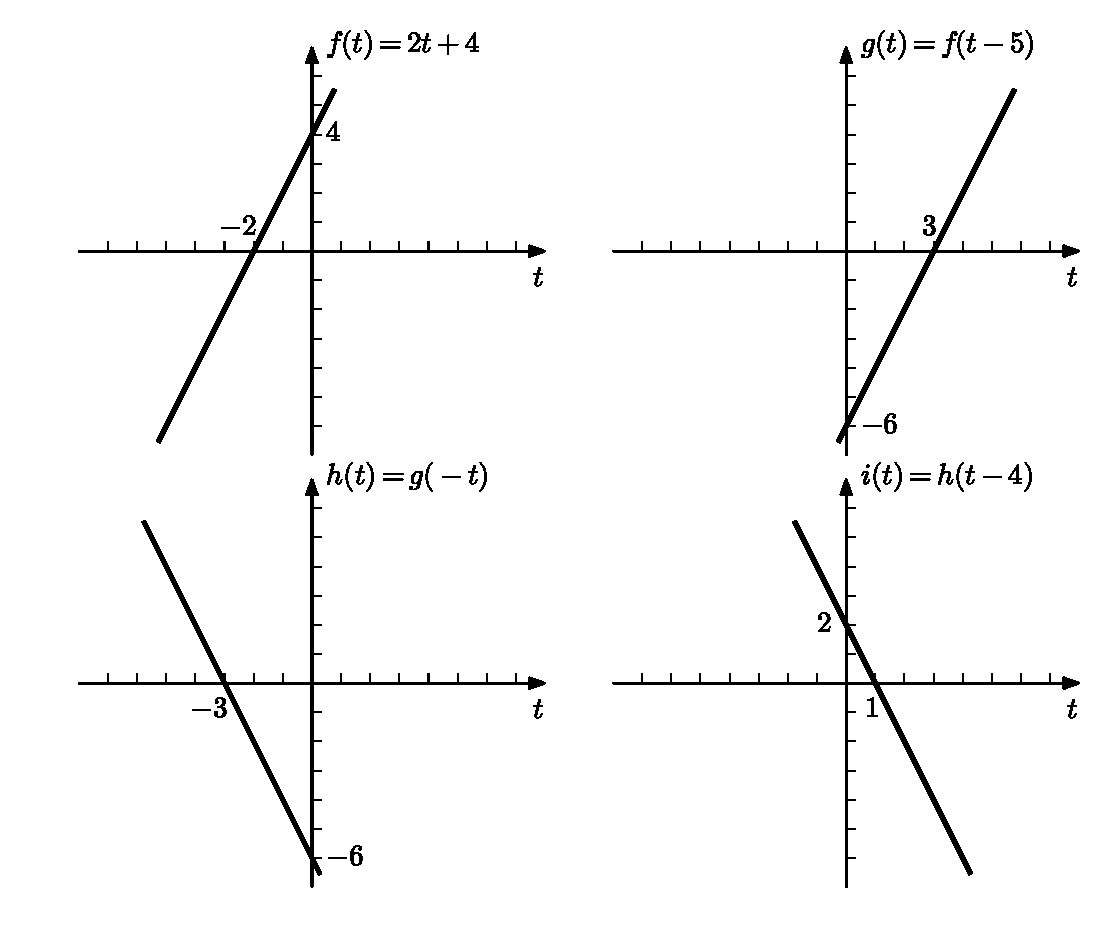
\includegraphics[width=0.9\columnwidth]{figuras/function_transformations.eps}
\caption{\label{fig:function_transformations} Sucesión de transformaciones realizadas sobre la función \(f(t)=2t+4\). Se aplica un retardo temporal de 5, luego una inversión temporal y finalmente, un retardo temporal de 4. Un retardo temporal de \(T\) consiste en desplazar la gráfica a la derecha una cantidad \(T\). Una inversión temporal consiste en reflejar la gráfica respecto al eje de las ordenadas.}
\end{center}
\end{figure}

\paragraph{Nuevo desplazamiento temporal} Se considera ahora una función \(i(t)\) que consiste en un desplazamiento temporal de la función \(h(t)\) como sigue,
\[
 i(t)=h(t-4).
\]
Definida de esta forma, la expresión de \(i(t)\) es
\[
 i(t)=h(t-4)=-2(t-4)-6,
\]
resultando en
\begin{equation}\label{eq:i}
 i(t)=-2t+2.
\end{equation}
Se expresará a continuación la función \(i(t)\) en función de \(g(t)\). Teniendo en cuenta que \(h(t)\) se definió como una inversión temporal de \(g(t)\), \(h(t)=g(-t)\), se tiene que
\begin{equation}\label{eq:i_in_function_of_g}
 i(t)=h(t-4)=g(-(t-4)),
\end{equation}
donde se sustituyó \(t\) por \(t-4\) en \(g(-t)\). Sustituyendo \(t\) por \(-(t-4)\) en \(g(t)\) (ecuación \ref{eq:g}), resulta en
\[
 i(t)=g(-(t-4))=2(-(t-4))-6=-2t+2, 
\]
coincidiendo con el resultado de la ecuación \ref{eq:i}, lo que comprueba la ecuación \ref{eq:i_in_function_of_g}. La función \(i(t)\) es una inversión temporal seguida de un retardo de 4 de la función \(g(t)\), y se expresa como \(i(t)=g(-(t-4))\). En general, una inversión temporal seguida de un retardo \(T\) consiste en la transformación \(f(-(t-T))=f(T-t)\).

Finalmente, se quiere expresar \(i(t)\) en función de \(f(t)\). Como \(g(t)=f(t-5)\), se tiene que
\[
 i(t)=h(t-4)=g(-(t-4))=f(-(t-4)-5),
\]
donde sobre \(f\) se realizaron las transformaciones retardo de 5, luego una inversión temporal y finalmente un retardo de 4. Generalizando, la transformación retardo de \(T_0\), seguida de una inversión temporal, seguida de un retardo de \(T_1\) es \(f(-(t-T_1)-T_0)\).

Con los mismos argumentos, es fácil ver que si sobre \(f(t)\) se realizan las transformaciones de inversión temporal, retardo de \(T\) y otra inversión temporal, se tiene que,
\[
 g(t)=f(-t),\qquad h(t)=g(t-T),\qquad i(t)=h(-t),
\]
y por lo tanto,
\[
 i(t)=h(-t)=g(-t-T)=f(-(-t-T)),
\]
es decir,
\[
 i(t)=f(t+T),
\]
que equivale a un adelanto temporal de \(T\) de la función \(f(t)\).

\subsection{Resumen}

En el cuadro \ref{tab:function_transformations} se muestra la composición de \(f(t)\) correspondiente a algunas transformaciones.

\begin{table}[h]
 \begin{center}
\bgroup
\def\arraystretch{1.2}
\begin{tabular}{|c|c|}\hline
\textbf{Transformación} & \textbf{Composición de \(f(t)\)}  \\ \hline
Retardo \(T\) & \(f(t-T)\) \\ \hline
Inversión temporal & \(f(-t)\) \\ \hline
\begin{tabular}{@{}c@{}}Retardo \(T\) e\\inversión temporal \end{tabular} & \(f(-t-T)\)\\ \hline
\begin{tabular}{@{}c@{}}Inversión temporal \\y retardo \(T\)\end{tabular} & \(f(-(t-T))\)\\ \hline
\begin{tabular}{@{}c@{}}Retardo \(T_0\), inversión\\temporal y retardo \(T_1\) \end{tabular} & \(f(-(t-T_1)-T_0)\)\\ \hline
\begin{tabular}{@{}c@{}}Inversión temporal, retardo \(T\)\\e inversión temporal \end{tabular}  & \(f(t+T)\)\\ \hline
\end{tabular}
\egroup
\end{center}
\caption{\label{tab:function_transformations} Algunas transformaciones de funciones.}
\end{table}

\section{Operación de convolución} 

A continuación se comentan aspectos específicos del cálculo de la convolución, operación que se definió como
\[
 (f*g)(t)=\int _{-\infty }^{\infty }f(\tau )\,g(t-\tau )\,d\tau.
\]
Debido a que la variable de integración es \(\tau\), el resultado es una función de variable \(t\), como se explicita en el lado izquierdo de la ecuación. La integral debe resolverse para cada valor de \(t\in\mathbb{R}\). Para esto, para calcular el resultado para un valor de \(t\) en particular, se fija \(t\) a ese valor y se considera que la variable independiente de las funciones \(f\) y \(g\) que participan en la convolución es \(\tau\). Por ejemplo, si se aplica la convolución entre \(f(t)\) y \(g(t)\), se cambia el nombre de la variable \(t\) a \(\tau\), resultando en las funciones \(f(\tau)\) y \(g(\tau)\). En la integral, el argumento de la función \(g\) es \(g(t-\tau)=g(-(\tau-t))\). Teniendo en cuenta que \(\tau\) es la variable y \(t\) es fijo, esto corresponde a una inversión temporal seguida de un retardo de \(t\), como se indica en el cuadro \ref{tab:function_transformations}. Por lo tanto, hay que invertir temporalmente a \(g(\tau)\), obteniendo \(g(-\tau)\), y luego retardarla una cantidad \(t\), obteniendo \(g(t-\tau)\).

\section{Convolución entre funciones transformadas}

\subsection{Convolución con una función retardada}

En la sección \ref{sec:definition} se mencionó que \(f(t)*g(t-T)\) es equivalente a \((f*g)(t-T)\) mientras que \(f(t-T)*g(t-T)\) es equivalente a \((f*g)(t-2T)\). A continuación se demostrarán ambas igualdades.

Se quiere calcular la convolución entre \(f(t)\) y \(g(t-T)\). Formalmente, la operación se expresa como
\[
 \left({f}*(\tau_{T}g)\right)(t),
\]
donde \(\tau_Tg\) es la transformación de retardo temporal, definida como
\[
 (\tau_{T}g)(t)=g(t-T),
\]
pero por claridad, se empleará la notación usada en ingeniería, \(f(t)*g(t-T)\). Para plantear la integral, se cambia el nombre de la variable de las funciones \(f\) y \(g\) a \(\tau\), obteniendo \(f(\tau)\) y \(g(\tau-T)\). Luego, cualquiera de las funciones se invierte temporalmente y se retarda una cantidad \(t\). Si se elige la función \(g\), la inversión temporal conduce a \(g(-\tau-T)\), y el retardo \(t\) a \(g(-(\tau-t)-T)=g(t-T-\tau)\). Por lo tanto,
\begin{align*}
 f(t)*g(t-T)&=\int _{-\infty }^{\infty }f(\tau)\,g(t-T-\tau)\,d\tau \\
   &=(f*g)(t-T),
\end{align*}
donde la segunda igualdad surge de observar que la integral es la definición de la convolución evaluada en \(t-T\).

Como indica la definición dada por la ecuación \ref{eq:convolution_definition}, la operación de convolución es conmutativa, y por lo tanto, el resultado sería el mismo si la inversión temporal y el retardo se hubiera aplicado sobre la función \(f\). Como antes, al realizar el cambio de nombre de la variable de las funciones, se obtiene \(f(\tau)\) y \(g(\tau-T)\), y la inversión temporal y retardo de \(f\) conduce a \(f(-(\tau-t))=f(t-\tau)\). Así,
\begin{align*}
 f(t)*g(t-T)&=\int _{-\infty }^{\infty }f(t-\tau)\,g(\tau-T)\,d\tau \\
   &\overset{(a)}{=}-\int_{\infty }^{-\infty }f(u)\,g(t-T-u)\,du \\
   &\overset{(b)}{=}\int_{-\infty }^{\infty }f(\tau)\,g(t-T-\tau)\,d\tau \\
   &=(f*g)(t-T),
\end{align*}
donde en \((a)\) se realizó el cambio de variable de integración \(u=t-\tau\) y en \((b)\) se invirtieron los límites de integración. Siguiendo un razonamiento análogo, es fácil ver que se cumple que
\[
 f(t)*g(t-T) = f(t-T)*g(t) = (f*g)(t-T).
\]

Se calculará ahora la convolución en el caso en que las dos funciones estén retardadas, esto es, \(f(t-T_0)*g(t-T_1)\). Al cambiar el nombre de la variable se obtiene \(f(\tau-T_0)\) y \(g(\tau-T_1)\), y al invertir temporalmente y retardar una de ellas, digamos \(g\), queda \(g(-(\tau-t)-T_1)\). Entonces,
\begin{align*}
 f(t-T_0)*g(t-T_1)&=\int_{-\infty }^{\infty }f(\tau-T_0)\,g(-(\tau-t)-T_1)\,d\tau \\
   &\overset{(a)}{=}\int_{-\infty }^{\infty }f(u)\,g(t-T_0-T_1-u)\,du \\
   &\overset{(b)}{=}(f*g)(t-(T_0+T_1)),
\end{align*}
donde en \((a)\) se realizó el cambio de variable de integración \(u=\tau-T_0\) y en \((b)\) se notó que la integral es la definición de la convolución evaluada en \(t-(T_0+T_1)\). En el caso en que \(T_0=T_1=T\), se obtiene que
\[
 f(t-T)*g(t-T)=(f*g)(t-2T).
\]

\subsection{Convolución con la delta de Dirac}

La distribución delta de Dirac es la identidad de la operación de la convolución, ya que
\begin{align*}
 f(t)*\delta(t)&\,=\int_{-\infty }^{\infty }f(\tau)\,\delta(t-\tau)\,d\tau \\
   &\overset{(a)}{=}\int_{-\infty }^{\infty }f(\tau)\,\delta(\tau-t)\,d\tau \\
   &\overset{(b)}{=}f(t),
\end{align*}
donde en \((a)\) se empleó que la función delta de Dirac es par, es decir, \(\delta(t)=\delta(-t)\) y en \((b)\) se usó una propiedad de la delta referida usualmente como ``sifting property''\footnote{\url{http://mathworld.wolfram.com/SiftingProperty.html}}.

Como consecuencia, el efecto de convolucionar una función con una delta desplazada en el tiempo, es desplazar a la función en el tiempo la misma cantidad, es decir,
\[
 f(t)*\delta(t-T)=f(t-T).
\]
Para demostrarlo, hay que plantear la integral de la definición, que implica cambiar el nombre de la variable de las funciones del integrando a \(\tau\) e invertir temporalmente y retardar una cantidad \(t\) una de ellas. Si se elige la delta, al cambiar el nombre de la variable e invertir temporalmente, se obtiene \(\delta(-\tau-T)\) y al retardar \(t\) queda \(\delta(-(\tau-t)-T)\). De esta forma, la integral queda
\begin{align*}
 f(t)*\delta(t-T)&=\int_{-\infty }^{\infty }f(\tau)\,\delta(-\tau+(t-T))\,d\tau \\
        &=\int_{-\infty }^{\infty }f(\tau)\,\delta(\tau-(t-T))\,d\tau \\
        &=f(t-T),
\end{align*}
donde se usaron las mismas propiedades que en el caso anterior.

\subsection{Convolución con una función invertida temporalmente}

Se considera ahora el caso en que se quiere calcular la convolución cuando una de las funciones está invertida temporalmente, esto es, \(f(t)*g(-t)\). Como ya se explicó, hay que cambiar el nombre de la variable a \(\tau\) obteniendo \(f(\tau)\) y \(g(-\tau)\), y luego \(g\) se invierte temporalmente y se retarda \(t\), obteniendo \(g(\tau-t)\). Por lo tanto,
\begin{align*}
 f(t)*g(-t)&=\int_{-\infty }^{\infty }f(\tau)\,g(\tau-t)\,d\tau \\
           &=\int_{-\infty }^{\infty }f(\tau+t)\,g(\tau)\,d\tau.
\end{align*}

Una función importante en procesamiento de señales es la función de autocorrelación de una señal, que se obtiene al convolucionar la señal con si misma invertida temporalmente. Así, la función de autocorrelación \(R_{ff}(t)\) de la señal \(f(t)\) se define como
\[
 R_{ff}(t)=(f*g_{-1}({\overline{f}}))(t),
\]
donde \(\overline{f}\) representa el complejo conjugado de \(f\) y \(g_{-1}\) la transformación de inversión temporal, es decir, \({\displaystyle g_{-1}(f)(t)=f(-t)}\). En la notación mas informal de la convolución empleada en ingeniería, esto se expresa como
\[
 R_{ff}(t)=f(t)*\overline{f}(-t),
\]
y de forma análoga al razonamiento realizado previamente, la integral es
\begin{align*}
 R_{ff}(t)&=f(t)*\overline{f}(-t)\\
          &=\int_{-\infty }^{\infty }f(\tau)\,\overline{f}(\tau-t)\,d\tau \\
          &=\int_{-\infty }^{\infty }f(\tau+t)\,\overline{f}(\tau)\,d\tau.
\end{align*}

\bibliographystyle{ieeetr}
% \bibliography{convolution_considerations}

\end{document}
